\documentclass[a4paper]{article}

%% Language and font encodings
\usepackage[english]{babel}
\usepackage[utf8x]{inputenc}
\usepackage[T1]{fontenc}
\usepackage{float}

%% Sets page size and margins
\usepackage[a4paper,top=3cm,bottom=2cm,left=3cm,right=3cm,marginparwidth=1.75cm]{geometry}

%% Useful packages
\usepackage{amsmath}
\usepackage{graphicx}
\usepackage[colorinlistoftodos]{todonotes}
\usepackage[colorlinks=true, allcolors=blue]{hyperref}
\usepackage{csquotes}
\usepackage{comment}
\usepackage{authblk}

\setlength{\parindent}{0em}
\setlength{\parskip}{1em}

\title{Predicting syntactic/semantic sentence frames from GLoVe vectors for verbs}
%this is not a great title, suggestions welcome heres a change

\author[1]{Kyle Sarent}
\author[2]{Melissa Kline}
\author[2]{Idan Blank}
\author[3,4]{Evelina Fedorenko}

\affil[1]{Harvard University}
\affil[2]{Department of Brain \& Cognitive Sciences, Massachusetts Institute of Magic}
\affil[3]{Massachusetts General Hospital}
\affil[4]{Harvard Medical School}

\begin{document}
\maketitle

\begin{abstract}
IN OUTLINE FORM

(0) While computational models of semantics that are based on purely distributional information have done well (CITES), semantic theories predict a role for frame-level representations, and these may explain why verb semantics are so hard. What are these frames and where do they come from? 

(1) Glove predicts frames pretty well!

(2) Ooh \... glove contains much more than just the frames, aka frames explain a tiny amount of GLOVE variance. 

(2a) Glove predicts frames, but frames don't predict glove. This is sensible from a linguistic preference. 

(3) So, what are human judgments? Some kind of combination of large distributional information (GLOVE) and structured semantic knowledge (VerbNet)? Maybe so! Here is SimVerb, which tells us directly how similar ppl find verbs.  Verbnet thinks those same verbs are X similar, while Glove thinks they are Y similar. These 3 similarity matrices compare LIKE SO, suggesting a possible role for explicit frame representations in human language, and that NL researchers should take further looks at VerbNet. 

\end{abstract}

This is an intro, stating what we are doing, what we'll set out to prove, and the bullet-point results. It's verb short. 

\section{Background}
\subsection{Verbs and argument structure}
Nouns are different from verbs
Verbs appear in certain frames
There are lots of theories as to why this is, or how to describe them, but the basic insight is that clustering by semantics 


%Kyle please format the following as a nice 2-column table or set of examples
\begin{figure}[H]
\centering
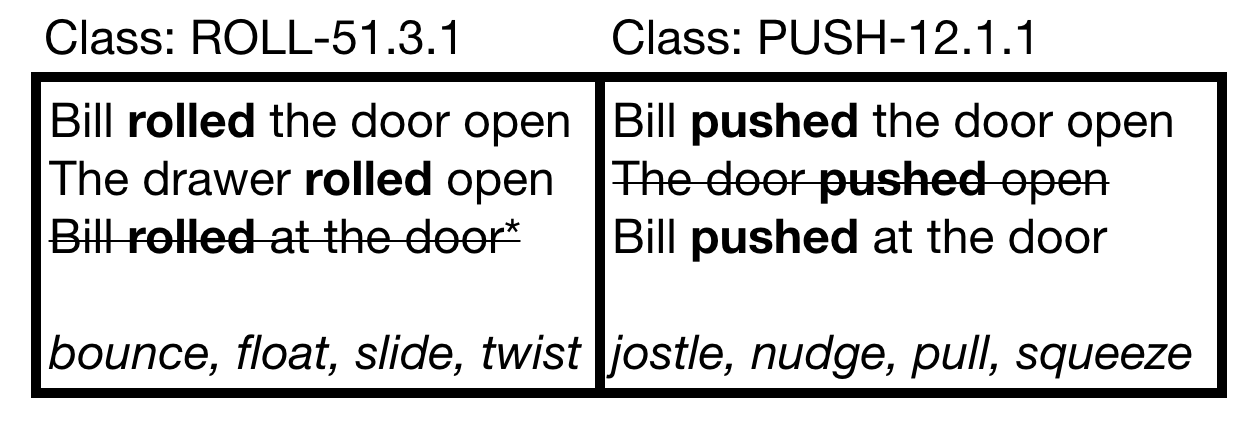
\includegraphics[width=0.5\textwidth]{VerbTable.png}
\caption{\label{fig:frog} Two verb classes from VerbNet (Palmer, CITATION), showing a subset of frames that are used to identify the classes, and examples of verb in that class.) No semantic criteria are used to generate the classes, but the verbs nevertheless share aspects of meaning.  *Note that this sentence is ungrammatical in the \emph{conative reading} (Bill attempted to roll the door but didn't move it, in parallel with "Bill pushed at the door.") The only grammatical interpretation is the \emph{locative reading} where Bill himself rolls towards the door. }
\end{figure}


Levin (1993) developed the notion of a verb class. This classification was extended and enriched by Verbnet, a database of about 8000 verb/class instances. The website of VerbNet describes a verb class:

\begin{displayquote}
“Each verb class in VN is completely described by thematic roles, selectional restrictions on the arguments, and frames consisting of a syntactic description and semantic predicates with a temporal function, in a manner similar to the event decomposition of Moens and Steedman (1988).”
\end{displayquote}

We are interested in demonstrating that GLoVe encodes syntax information; thus, the most natural thing to try and predict are the frames a verb fits into. It is worth noting that in VerbNet, whether or not a verb fits in a frame is true or false, with no gray area - in practice, such judgments by humans are much fuzzier. 


Any verb in VerbNet belongs to some number of classes, and each class expresses some number of the 291 frames. Suppose we number the frames $f_1... f_{291}$. The notion of a “binary frame vector” associated to a verb is as follows: Suppose a verb vhas associated binary frame vector $v$, then we assign the following value to entry $i$ of the frame vector:

	\[ v_i =1  \text{if $v$ belongs to frame $i$ in any of its class instantiations, and 0 otherwise} \]

\subsection{Distributional models of verb semantics}

IDAN/KYLE WRITE - can be short, focus on what's different about this - primarily, we treat verbs just like any other words. Describe/cite what Glove is. This is the section to head off objections about sense/POS disambiguation as well - say whether we're using a Glove version that does, acknowledge any limitation, and move on. )

On the other hand, for most of the verbs in VerbNet, we have GLoVe vectors. For this project, I wanted to make use of distributional information from Wikipedia and Twitter - thus, GLoVe vectors from both were concatenated to form a 400-dimensional vector of real numbers that encodes its distributional information. 

\section{Predicting VerbNet frames from GLoVe, and vice versa}

\subsection{Summary of the prediction task - VerbNet from GLoVe}

We can reduce from the problem of recovering verb syntax from GLoVe to learning a good approximate mapping from the 400-dimensional GLoVe space to the 291-dimensional space of binary frame vectors. In the field of machine learning, this is known as a multi-label classification problem.

We’ll randomly shuffle the set of verbs for which we have both GLoVe vectors and frame vectors into a training set of 2949 verbs, and a validation set of 737 verbs, i.e. the standard 80/20 training/validation split for most machine learning problems. By learning a mapping from glove vectors to frames on the training data and checking its precision (see part 2) on the validation data, we will attempt to demonstrate that we can in fact successfully recover syntax information from GLoVe.

One of the simplest possible models was chosen for classification: a logistic regression model. Since a logistic regression model is a binary classifier, and we are interested in 291 classification problems, we simply concatenate and separately train 291 independent logistic classifiers to predict the frame vector of a verb from its GLoVe vector.

An advantage of a logistic regression model is that its transparency will allow us to directly examine the weights on each dimension of GLoVe - in short, it may be able to find which dimensions of GLoVe are most diagnostic, for syntax purposes.

To ensure robust predictions, positive training examples in both training and testing sets, and to simplify the problem of disentangling the data into training and testing sets such that this latter condition is satisfied, all frames with 5 or fewer positive training examples have been excluded from our prediction task. Since there are 232 frames with more than 5 positive training examples, we restrict our investigation to these frames (for the time being).

\subsubsection{Discussion of Results}

Since we are evaluating hundreds of independent binary classifiers, the Area Under the Receiver Operating Curve (AUROC) seems a fair benchmark for our model. The receiver operating curve of a binary classifier is essentially the true positive rate of the classifier, plotted against its false positive rate. That is, the probability it will correctly classify a positive example as a function of the probability it will incorrectly classify a negative example. When these points are joined they form a curve, and the area under it, or AUROC, measures the effectiveness of a binary classifier by giving a number between .5 and 1.0 that measures the strength of the tradeoff between false positives and true positives - at .5, a model is no better than a random classifier. At 1.0, the model classifies all training examples perfectly. 

After fitting the 232 logistic regressions on the training data, we now consider their performance on the testing data. We can plot the receiver operating curves atop one another as below. They appear vary widely, but there is no mistaking that the average predictive strength is well above a random classifier. However, some spuriously trained models do quite poorly - take a look at the curves that fall below the random classifier benchmark line $y = x$.  

\begin{figure}[H]
\centering
\includegraphics[width=0.5\textwidth]{AUC_plot5.png}
\caption{\label{fig:frog} 232 frames with minimum 5 training examples, AUC average = .8431}
\end{figure}

It is easy to see that, on average, predicting frames from GLoVe vectors using a logistic regression classifier does better than random chance. But there is a lot of variance in how good the model is for different frames. Let's see what happens when we raise the threshold for training examples.

\begin{figure}[H]
\centering
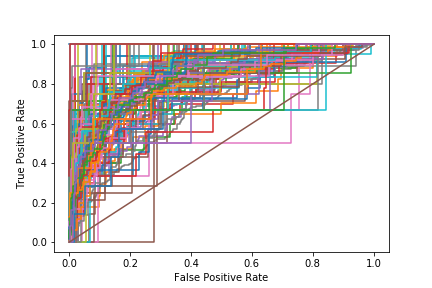
\includegraphics[width=0.5\textwidth]{auc_plot15.png}
\caption{\label{fig:frog} 155 frames with minimum 15 training examples, AUC average = .8421}
\end{figure}

\begin{figure}[H]
\centering
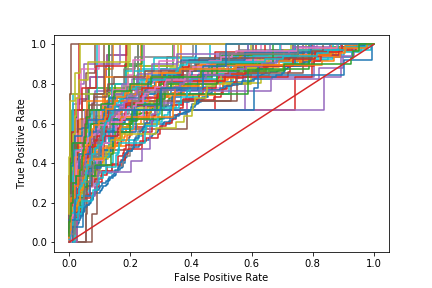
\includegraphics[width=0.5\textwidth]{auc_plot30.png}
\caption{\label{fig:frog} 93 frames with minimum 30 training examples, AUC average = .8409}
\end{figure}

\begin{figure}[H]
\centering
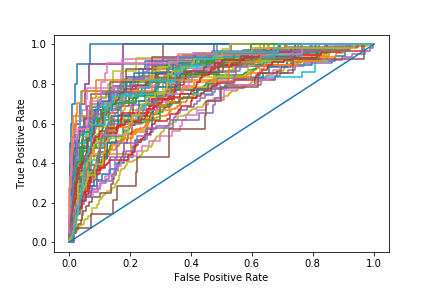
\includegraphics[width=0.5\textwidth]{auc_plot50.png}
\caption{\label{fig:frog} 60 frames with minimum 50 training examples, AUC average = .8111}
\end{figure}

It's clear from the above plots that model stability and performance goes up as a function of the number of training examples. What's encouraging is that AUC seems to stabilize as well. Let's take a look at a scatterplot of AUC against the number of training examples.

\begin{figure}[H]
\centering
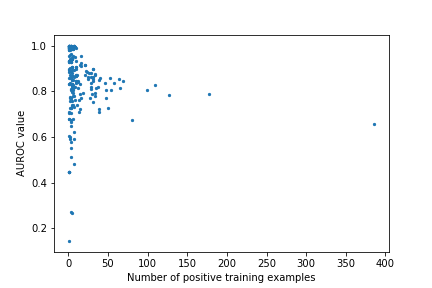
\includegraphics[width=0.5\textwidth]{auc_scatter5.png}
\caption{\label{fig:frog} }
\end{figure}

As training examples (the X-axis) increases, the spread in AUC tends to decrease, all the while stabilizing at around .75, confirming our hypothesis.

It seems clear that our model is predicting syntax reasonably well from GLoVe vectors. How can we be sure we have not overfitted a model? For one, the training data was thrown away after model fitting, and all the results you see above are on the test set. This alone is reason to believe we have not overfitted to our data.

Suppose we scrambled the assignment of verbs to frames. Our model could still pick up on the distributional information of frames (e.g. this frame occurs 30\% of the time, so with a false positive tolerance of 70\% or more we should predict it always), but the GLoVe vector observations for a verb would be meaningless. How does such a model do? Let us examine their collective ROC plots. 

\begin{figure}[H]
	\centering
	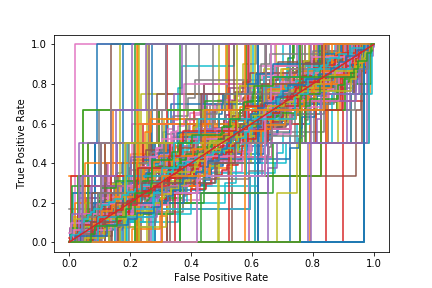
\includegraphics[width=0.5\textwidth]{auc_plot5rand.png}
	\caption{\label{fig:frog} }
\end{figure}

\begin{figure}[H]
	\centering
	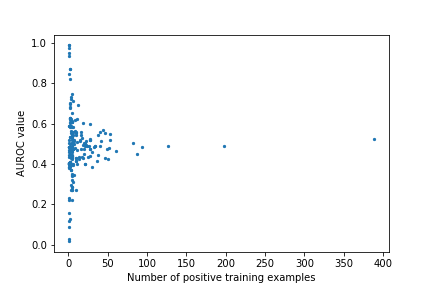
\includegraphics[width=0.5\textwidth]{auc_scatter5rand.png}
	\caption{\label{fig:frog} }
\end{figure}

These models perform no better than random chance. Indeed, it's clear in this case that 
\[  \lim_{\# \text{training examples} \rightarrow \infty} AUC = .5 \]
Which is as we expect for a collection of fundamentally random (uninformed) classifiers. This is good because it tells us GLoVe vectors give us frame information when (and only when) this information is correctly paired, which is another confirmation of our hypothesis.

\section{Modeling human similarity judgments from VerbNet and GLoVe}


\section{Diagnostic Verbs and Diagnostic Frames}

The following section describes my attempt to answer the following question: Which verbs and frames are the most "diagnostic?" Here, we take diagnostic to mean "explanatory" in the following sense - how can we pick a collection of frames and verbs that best represent their resepective datasets? In both cases, I have decided to use clustering to ensure maximal coverage of our dataset.

\subsection{Diagnostic Frame Clustering}

Unfortunately, clustering requires the space of frames to be endowed with a distance metric. There is not a canonical notion of "distance" between two frames, so I have decided that frames which occur in largely the same verbs should be "close" and frames which don't occur in the same verbs should be "far." There is a mathematically nice way for defining a distance metric on the space of finite sets - \textit{Jaccard distance}. This distance will capture the above, naive intuition about frame distance.

Consider two frames $f_1$ and $f_2$ and the set of verbs in which they appear, $V_1$ and $V_2$. The $\textit{Jaccard}$ distance between $V_1$ and $V_2$ is defined
\[ d_J(V_1, V_2) =  1 - \frac{|V_1 \cap V_2|}{|V_1 \cup V_2|} \]
That this constitutes a formal distance metric on the space of finite sets is out of scope, but this fact is required to justify clustering. Nevertheless, it is easy to see that dissimilar frames will be "far apart." If the set of verbs in which both frame $f_1$ and $f_2$ appear is empty,  $d_J = 1 - \frac{0}{|V_1 \cup V_2|} = 1$. Likewise if they appear in only the same verbs, their distance is zero (for all practical purposes, the frames are identical)

With a distance metric, we can run spectral clustering (preferred over standard K-means clustering because it can detect non-Euclidean clusters like long, thin agglomerations) with as many clusters as we like.

\subsection{Diagnostic Verb Clustering}

Due to computational limitations, spectral clustering is infeasible for the several thousand verbs for which I have GLoVe vectors, even with PCA to reduce their dimensionality. Thus, simple K-means clustering was used to cluster verbs. 

\subsection{Diagnostic Table}

The purpose of determining a set of diagnostic frames and verbs is to construct a table $T$ that has columns labeled with frames and rows labeled with verbs, such that the entry in row $v$ and column $f$ is "True" if verb $v$ fits into frame $f$, and false otherwise. With this table, validation of VerbNet and our logistic regression method on humans can be simplified.

We are motivated to produce a suitably rich table for human testing. On average, a verb fits into about 4.4 frames, so having no priors we could expect about $4.4/291 \approx 1.5\%$ of the entries in our table to be actual instances of a frame fitting into a verb, which is not ideal. We would like to push percentage $p_{true}$  higher so humans can maintain their focus in the verb/frame matching task. 

This is accomplished via the following randomized procedure after clustering the frames into $n_f$ clusters and the verbs into $n_v$ clusters. First, we pick a random frame from each frame cluster and a random verb from each verb cluster, to furnish a concrete set of $n_f$ diagnostic frames and a concrete set of $n_v$ diagnostic verbs. We then construct an $n_v \times n_f$ table as described above -- with rows labeled by verb and columns labeled by frames. Finally, we drop the $n_v / 2$ sparsest rows and the $n_f/2$ sparsest columns (in that order) to produce a smaller but richer $n_v/2 \times n_f/2$ table.

With the intent of producing a 50x25 table, we can start with 100 verb clusters and 50 frame clusters and, after clustering, run the procedure above until we get a suitably rich table, for example with $p_{true} \approx 10\%$. 
\begin{comment}

\subsection{Works Cited}

You can upload a \verb|.bib| file containing your BibTeX entries, created with JabRef; or import your \href{https://www.overleaf.com/blog/184}{Mendeley}, CiteULike or Zotero library as a \verb|.bib| file. You can then cite entries from it, like this: \cite{greenwade93}. Just remember to specify a bibliography style, as well as the filename of the \verb|.bib|.

You can find a \href{https://www.overleaf.com/help/97-how-to-include-a-bibliography-using-bibtex}{video tutorial here} to learn more about BibTeX.

We hope you find Overleaf useful, and please let us know if you have any feedback using the help menu above --- or use the contact form at \url{https://www.overleaf.com/contact}!

\bibliographystyle{alpha}
\bibliography{sample}

\end{comment}

\end{document}